\documentclass{beamer}
\usepackage{graphicx}

\mode<presentation>
{
  \usetheme{Frankfurt}
  \setbeamercovered{transparent}
}

\setcounter{tocdepth}{1}

\title[Water Compression]{Improved Data Compression of Molecular Dynamics of
  Water}

%\subtitle{}

\author{Keegan Smith
  \and Julian Kenwood
  \and Min-Young Wu}

\titlegraphic{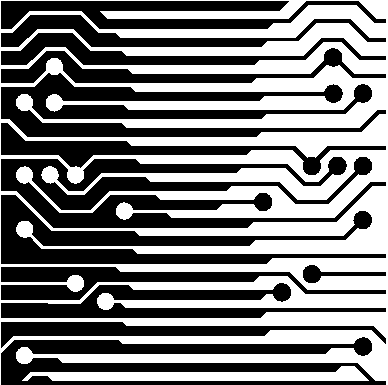
\includegraphics[height=16mm]{cslogo}}

\date{24 November 2009}

\institute[UCT]{Department of Computer Science \\ University of Cape Town}

\AtBeginSection[]
{
  \begin{frame}
    \frametitle{Outline}
    \tableofcontents[currentsection]
  \end{frame}
}

\begin{document}

\begin{frame}
  \titlepage
\end{frame}


% {{{
\section{Introduction}
\begin{frame}{Introduction}
  \begin{itemize}
  \item Molecular Dynamics Simulations are simulations representing the
    interactions of atoms over a period of time.

  \item Many such simulations contain a large amount of water molecules, often
    between 50\% to 90\% of the atoms are part of a water molecule.

  \item These simulations can represent a very large time period, so they can
    be very large: From $100$MB to $1$TB.

  \item The aim of our project was to develop compression schemes that are
    able to take advantage of this large amount of water.
  \end{itemize}
\end{frame}


\begin{frame}{Introduction}
  \begin{figure}
    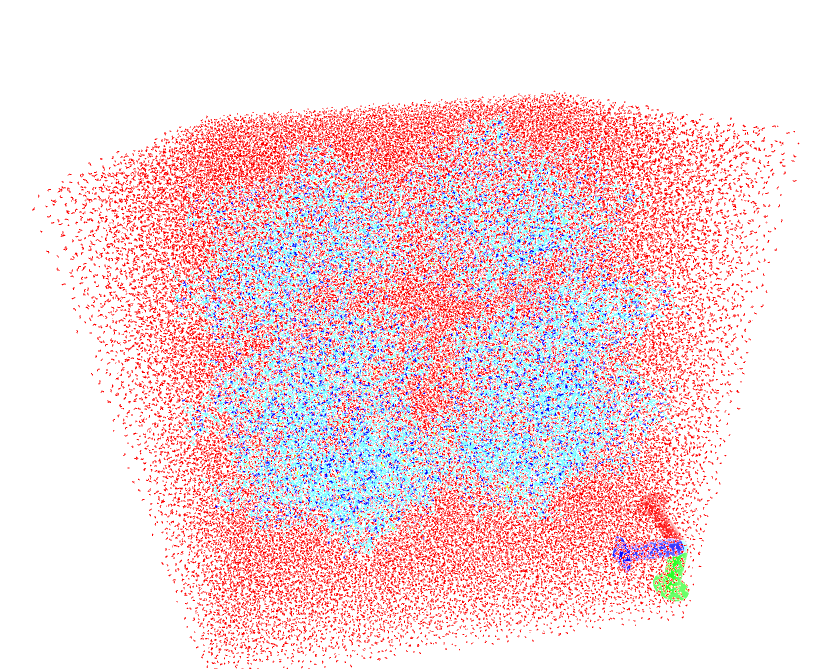
\includegraphics[width=0.5\textwidth]{julian-images/rabies.png}
    \caption{A Rabies Virus in water. There is a total of $450\,000$ atoms,
      68\% of which is water.}
  \end{figure}
\end{frame}
% }}}

\begin{frame}{Compression Process}
  % Julian: Explain that this is data flowing and make the distinction between
  % intraframe and interframe more clear.
  \begin{itemize}
   \item Dataflow for the compression process.
  \end{itemize}

  \begin{figure}
    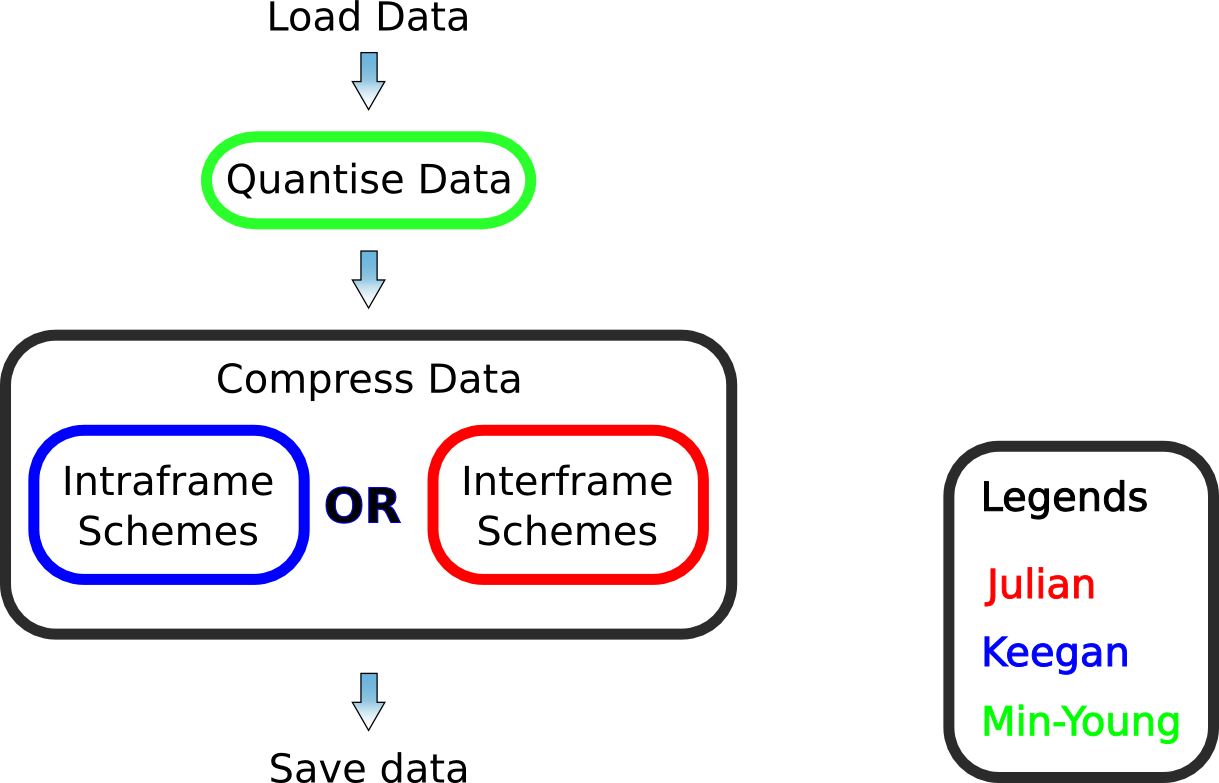
\includegraphics[width=0.9\textwidth]{legends.png}
  \end{figure}
\end{frame}


\section{Visualisations and Quantisation}

\begin{frame}{Visualisations}
% {{{
To examine the simulations, a number of visualisations were developed:
\begin{enumerate}

  \item Water Point
  \begin{itemize}
    \item Water molecules represented by points.
  \end{itemize}

  \item Ball-and-stick
  \begin{itemize}
    \item Atoms represented by spheres.
  \end{itemize}

  \item Metaballs
  \begin{itemize}
    \item Boundary between water and non-water regions extracted.
  \end{itemize}

  \item Water Cluster
  \begin{itemize}
    \item Water molecules are clustered together.
  \end{itemize}

  \item Quantisation Error
  \begin{itemize}
    \item Shows introduced quantisation error.
  \end{itemize}

\end{enumerate}
\end{frame}
% }}}

\begin{frame}{Visualisation}{Water Point}
% {{{
\begin{figure}
  \centering
  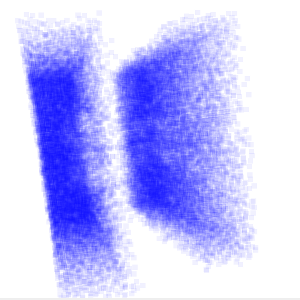
\includegraphics[width=55mm]{min-images/water-point.png}
  \caption{Each water molecule is represented by a single point.}
\end{figure}
\end{frame}
% }}}

\begin{frame}{Visualisation}{Ball-and-stick}
% {{{
\begin{figure}
  \centering
  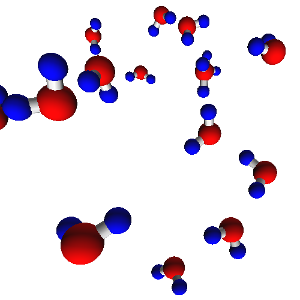
\includegraphics[width=55mm]{min-images/ball-and-stick.png}
  \caption{Molecules are represented by colour coded spheres, with the cylinders representing the bonds between atoms.}
\end{figure}
\end{frame}
% }}}

\begin{frame}{Visualisation}{Metaballs}
% {{{
\begin{figure}
  \centering
  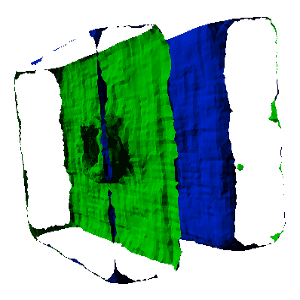
\includegraphics[width=55mm]{min-images/metaballs.png}
  \caption{The boundary between the water and non-water regions of the volume are extracted and rendered.}
\end{figure}
\end{frame}
% }}}

\begin{frame}{Visualisation}{Water Cluster}
% {{{
\begin{figure}
  \centering
  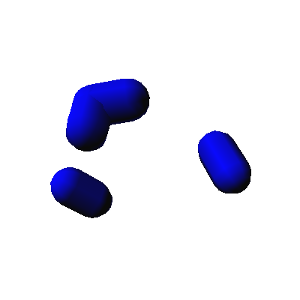
\includegraphics[width=55mm]{min-images/water-cluster.png}
  \caption{Water molecules within a cluster are joined together using cylinders.}
\end{figure}
\end{frame}
% }}}

\begin{frame}{Visualisation}{Quantisation Error}
% {{{
\begin{figure}
  \centering
  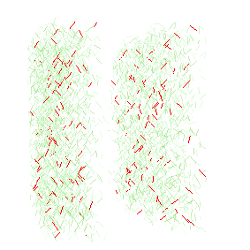
\includegraphics[width=55mm]{min-images/quantisation-error-line.png}
  \caption{The error introduced from quantisation is colour coded on a gradient.}
\end{figure}
\end{frame}
% }}}

\begin{frame}{Quantisation}
% {{{
To aid compression, the floating point data is first converted to integer values.

\begin{figure}
  \centering
  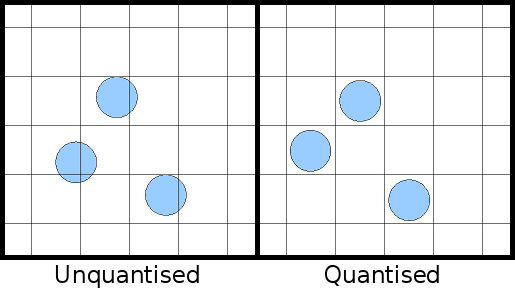
\includegraphics[width=75mm]{min-images/quantisation.png}
  \caption{Quantising point data can be seen as snapping points to a grid.}
\end{figure}
\end{frame}
% }}}

\begin{frame}{Quantisation Experiment}
% {{{

\begin{itemize}

  \item Quantisation causes a loss in data.

  \item Researchers will be visually examining the simulations, how much error is noticeable?

  \item A quantisation experiment was conducted to measure the perceptually visible effects of quantisation.

  \item Determine an appropriate level of quantisation, tradeoff between compression ratio and discarded data. \\ \

  \item What is the level of quantisation where the perceived differences between the original and quantised data are not significantly different.

\end{itemize}

\end{frame}
% }}}

\begin{frame}{Quantisation Effects}
% {{{
\begin{figure}
  \centering
  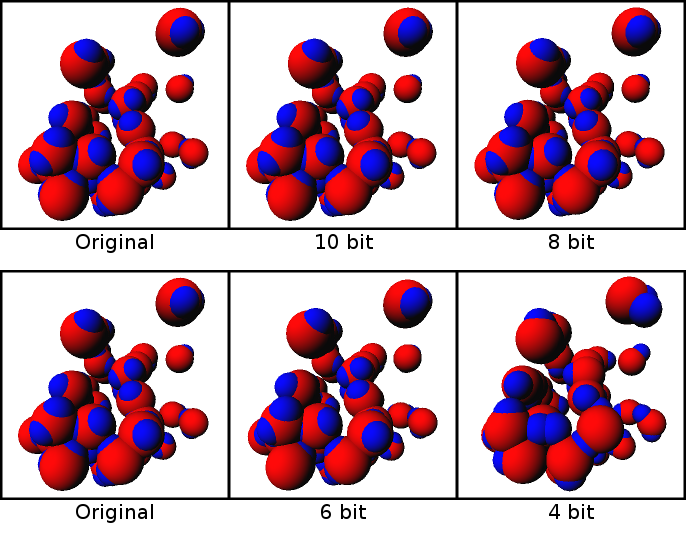
\includegraphics[width=70mm]{min-images/ball-and-stick-4680.png}
  \caption{Quantisation effects for the ball-and-stick visualisation.}
\end{figure}
\end{frame}
% }}}

\begin{frame}{Quantisation Effects}
% {{{
\begin{figure}
  \centering
  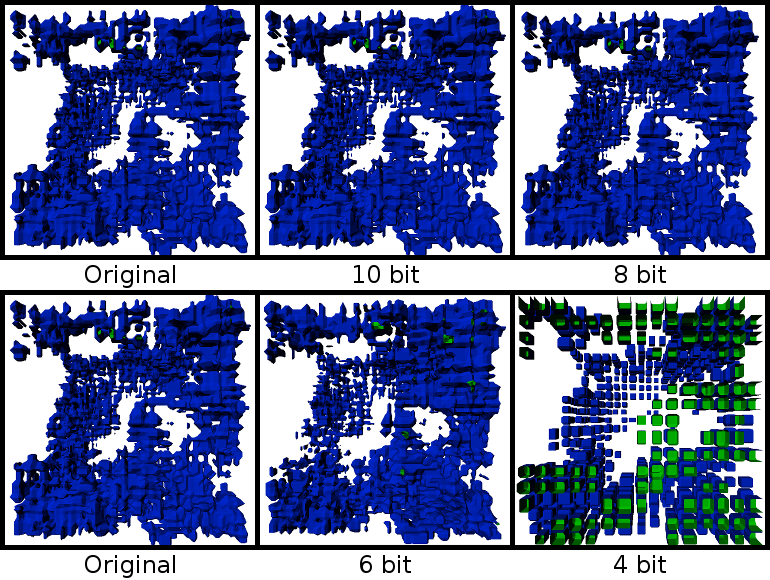
\includegraphics[width=70mm]{min-images/metaballs-4680.png}
  \caption{Quantisation effects for the metaballs visualisation.}
\end{figure}
\end{frame}
% }}}

\begin{frame}{Analysis of Quantisation Results}
% {{{
\begin{itemize}

  \item The datasets do \textbf{not} have a statistically significant effect \\
  {\footnotesize Which is \textbf{good}, all datasets were similary affected by quantisation.
  Friedman Test \textbf{p-value: $>$0.1}}

  % \item The data is normal \\
  % {\footnotesize Shapiro-Wilks Test \textbf{p-value: $<$0.01}}

  \item Quantisation has a statistically significant effect \\
  {\footnotesize ANOVA \textbf{p-value: $<$2.2e-16}}

  \item 8 and 10 bit quantisation are not statistically significantly different
  from each other \\
  {\footnotesize Ball-and-stick: \textbf{p-value of 0.7135299}} \\
  {\footnotesize Metaballs: \textbf{p-value of 0.9762546}}

\end{itemize}
\end{frame}
% }}}

\begin{frame}{Quantisation Results}
% {{{
\begin{figure}
  \centering
  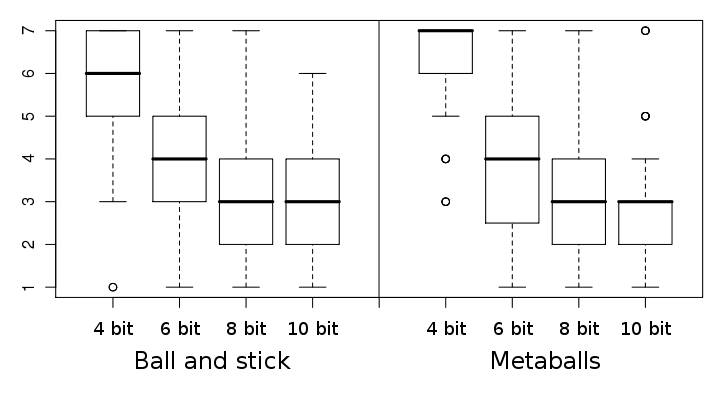
\includegraphics[width=100mm]{min-images/bm-boxplot.png}
  \caption{Box-and-whisker plot showing the ratings for each of the quantisation levels and visualisations.}
\end{figure}
\end{frame}
% }}}

\begin{frame}{Quantisation Results}
% {{{
\begin{figure}
  \centering
  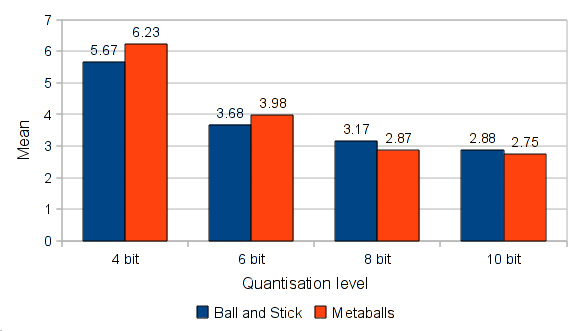
\includegraphics[width=100mm]{min-images/bm-means.png}
  \caption{Graph showing the mean ratings for each of the quantisation levels and visualisation techniques.}
\end{figure}
\end{frame}
% }}}


% {{{
\section{Intraframe}
\begin{frame}{What We Implemented}
  \begin{itemize}
    \item Reference Point Cloud Compressors
      \begin{itemize}
        \item Devillers and Gandoin
        \item Gumhold et.~al.
      \end{itemize}
    \item Reference General MD Compressor by Omeltchenko et.~al.~(Implemented
      by Julian)
    \item Reference compressor using quantisation and gzip
    \item Our own scheme is a predictive point cloud compressor which targets
      water.
  \end{itemize}
  \begin{figure}[h]
    \centering
    \begin{tabular}{ccccc}
        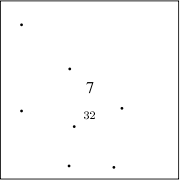
\includegraphics[width=0.25\textwidth]{keegan-images/dg1}
      & $\to$
      & 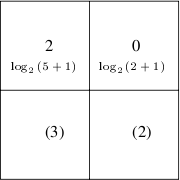
\includegraphics[width=0.25\textwidth]{keegan-images/dg2}
      & $\to$
      & 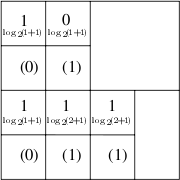
\includegraphics[width=0.25\textwidth]{keegan-images/dg3}
    \end{tabular}
  \end{figure}
\end{frame}
\begin{frame}{Water Compression Scheme}{Predictors}
  \begin{figure}[h]
    \centering 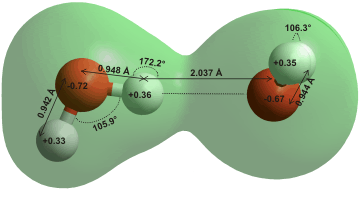
\includegraphics[width=0.6\textwidth]{keegan-images/h402}
  \end{figure}
  \begin{figure}[h]
    \centering 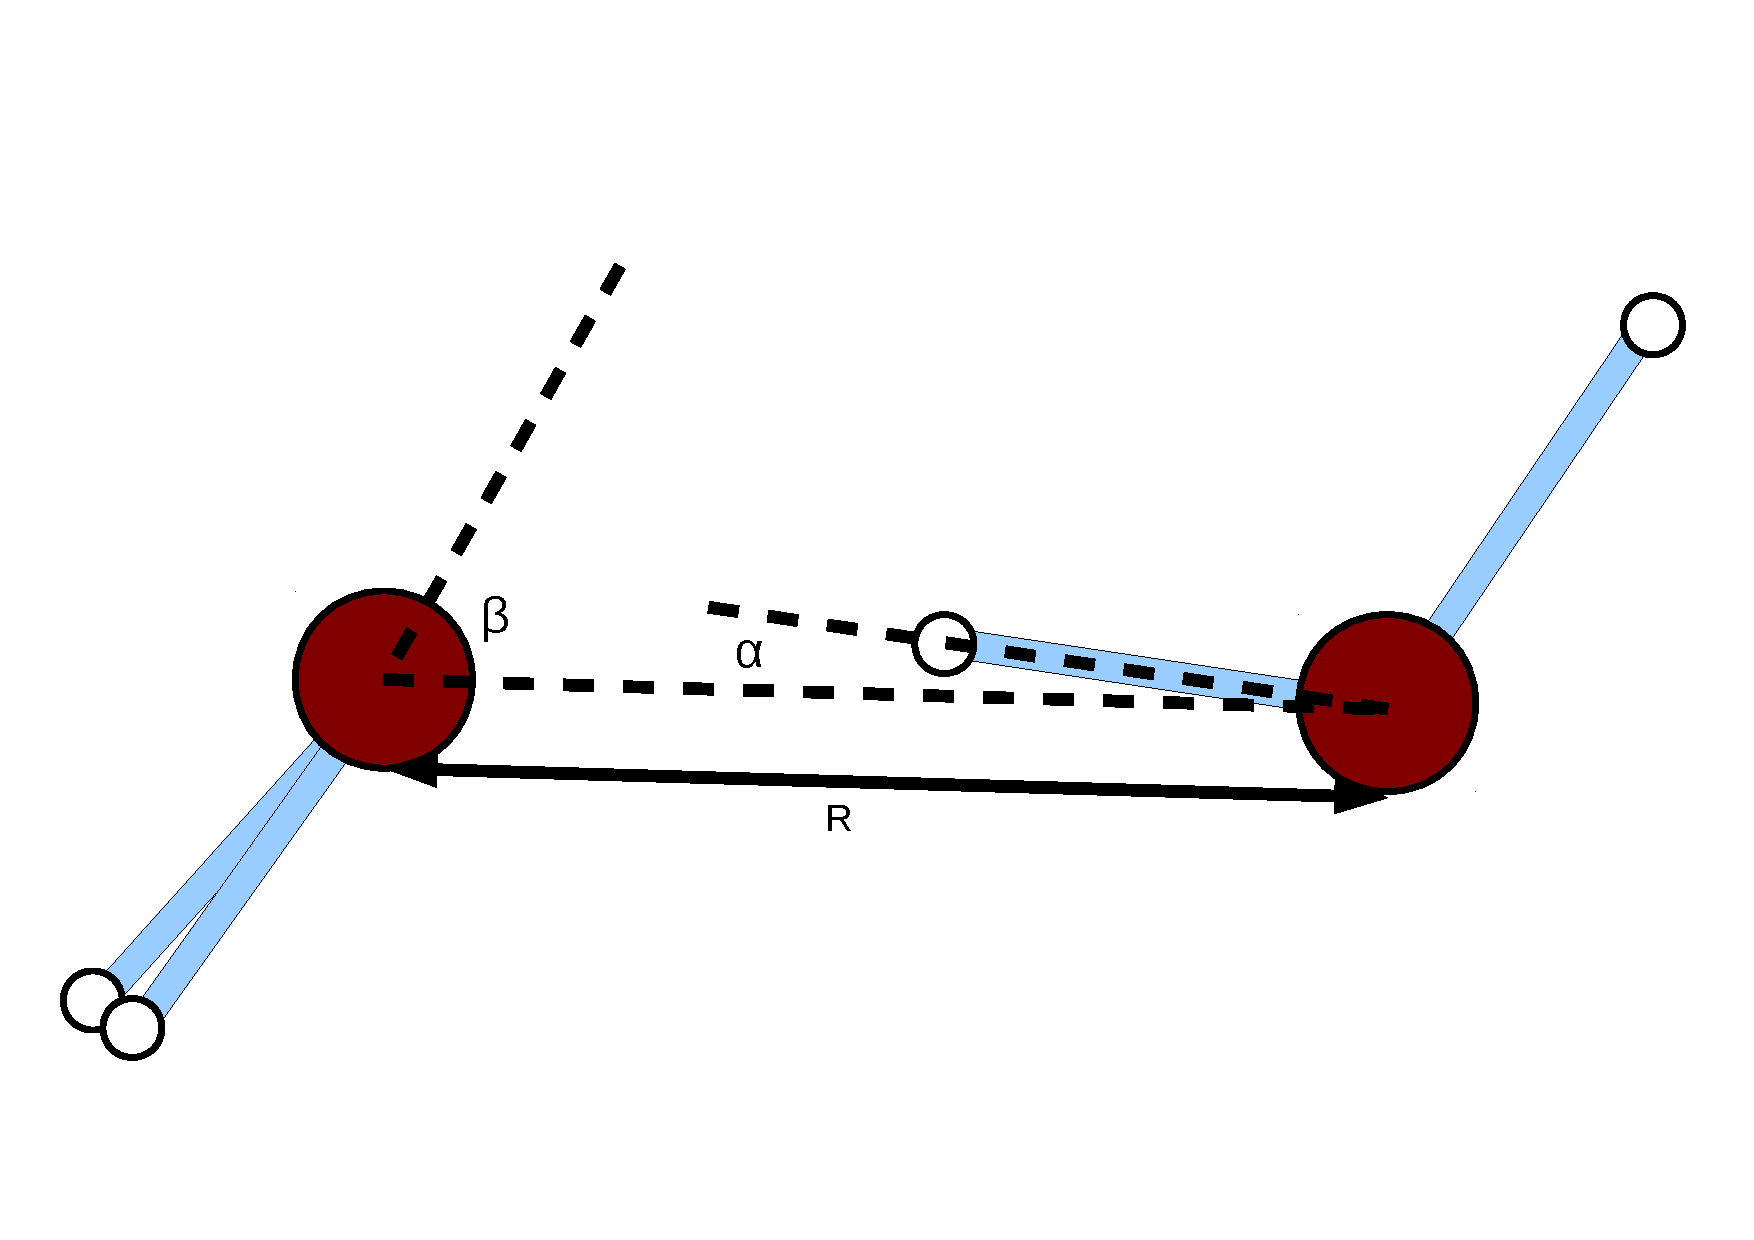
\includegraphics[trim = 10mm 30mm 10mm 45mm, clip,
      width=0.6\textwidth]{keegan-images/dimer-angle}
  \end{figure}
\end{frame}

\begin{frame}{Water Compression Scheme}{High-level Overview}
  \begin{enumerate}
  \item Separate the water and non-water atoms and compress separately.
  \item Create graph of water molecules.
  \item Create a spanning tree from the graph.
  \item Encode the tree, predictor used and residuals. This is done in BFS
    order.
  \end{enumerate}
\end{frame}

\begin{frame}{Permutation Encoding}{Problem}
  \begin{itemize}
  \item Many of the schemes (including our scheme) do not preserve the order
    of the points in the file.
  \item For example in Devillers and Gandoin
    \[ [ (1, 2), (1, 3), (0, 0), (2, 3), (2, 2), (0, 2), (1, 1) ] \]
    when decompressed becomes
    \[ [ (0, 0), (1, 1), (0, 2), (1, 2), (1, 3), (2, 2), (2, 3) ] \]
  \item The file format requires the original order of the points to be
    recovered.
  \item Encoding the order of the points became a significant portion of the
    compressed file.
  \end{itemize}
\end{frame}

\begin{frame}{Permutation Encoding}{Solution}
  \begin{itemize}
  \item We thought up and explored five different techniques.
  \item We derived the lower bound for the worst case performance of a general
    permutation encoder.
    \begin{equation*}
      \displaystyle\sum^{N}_{i=1} \log_2(i)
    \end{equation*}
  \item We showed that our scheme, \textbf{optimal}, encodes at roughly the
    lower bound.
  \item Empirically our scheme, \textbf{delta}, performed best since its worse
    case is unlikely to occur.
  \end{itemize}
\end{frame}

\begin{frame}{Results}
  \begin{figure}[h]
    \centering 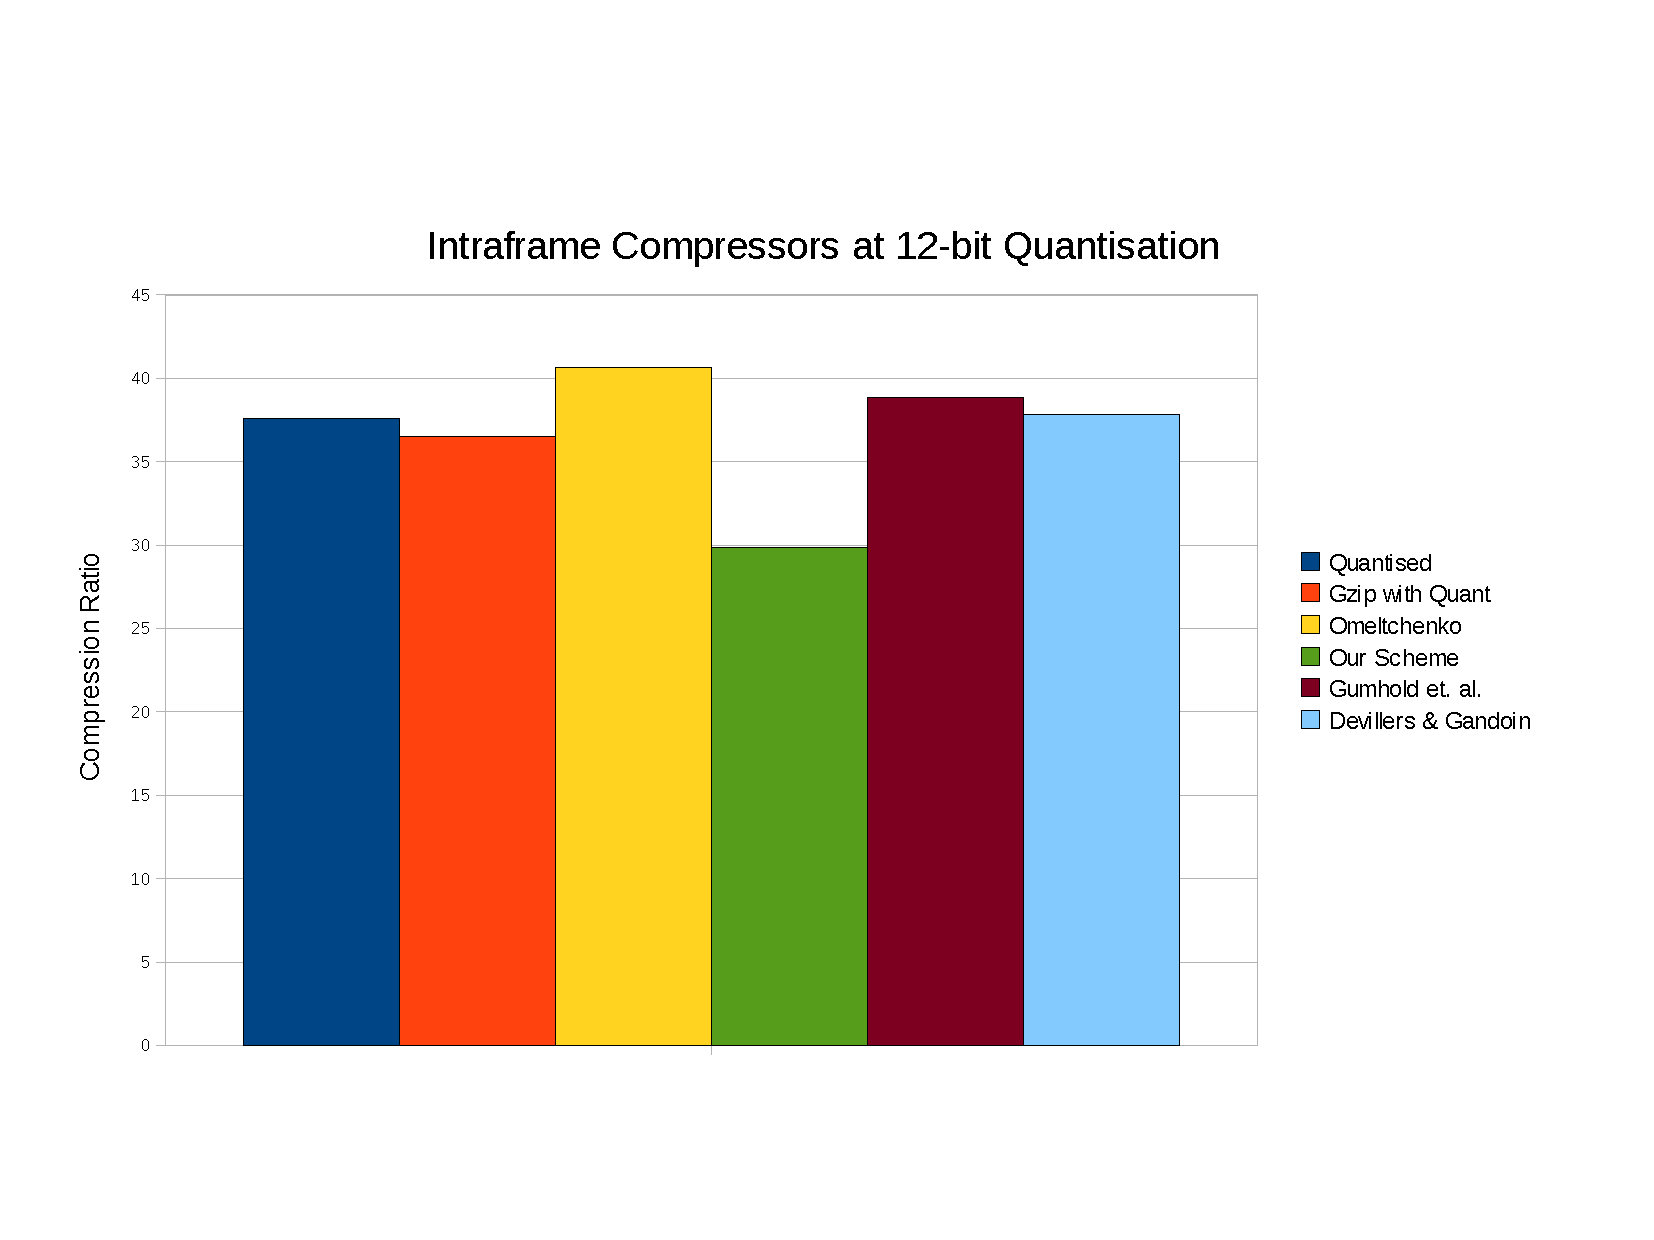
\includegraphics[trim = 10mm 30mm 10mm 35mm, clip,
      width=0.9\textwidth]{keegan-images/results-average}
  \end{figure}
  \begin{itemize}
  \item In some test cases (with 100\% water), our scheme had a 11\% gain on
    the next best intraframe scheme.
  \end{itemize}
\end{frame}


\section{Interframe}

\begin{frame}{Overview}
\begin{itemize}
 \item Interframe Compression is a technique where atoms are compressed using
   knowledge about their previous positions.

 \item Five Interframe Compression schemes were implemented and tested:
 \begin{itemize}
   \item Polynomial Extrapolation
   \item Spline Extrapolation
   \item Smallest Error Encoding
   \item Common Error Encoding
   \item k-Nearest Neighbour Encoding
 \end{itemize}
\end{itemize}
\end{frame}

\begin{frame}{Polynomial Extrapolation}
  \begin{figure}[h]
    \centering 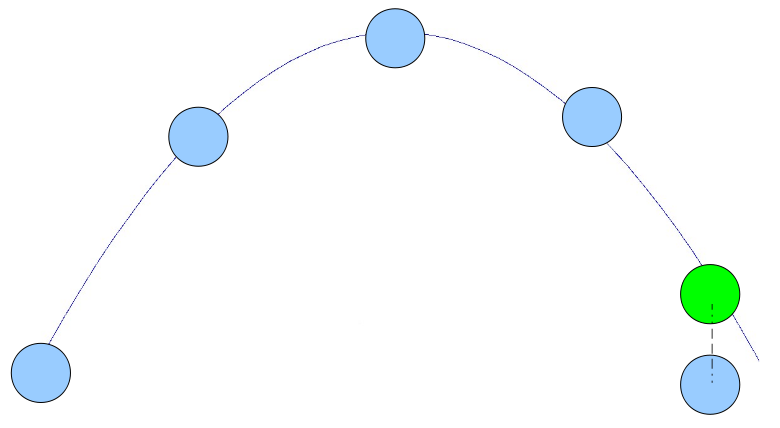
\includegraphics[width=0.6\textwidth]{julian-images/p1.png}
  \end{figure}
\begin{itemize}
 \item Uses the Lagrange Interpolation formula to construct a polynomial that
   passes through all of the previous atom positions.

 \item Using this polynomial, a prediction is made as to where the atom is
   likely to be.
\end{itemize}
\end{frame}

\begin{frame}{Spline Extrapolation}
  \begin{figure}[h]
    \centering 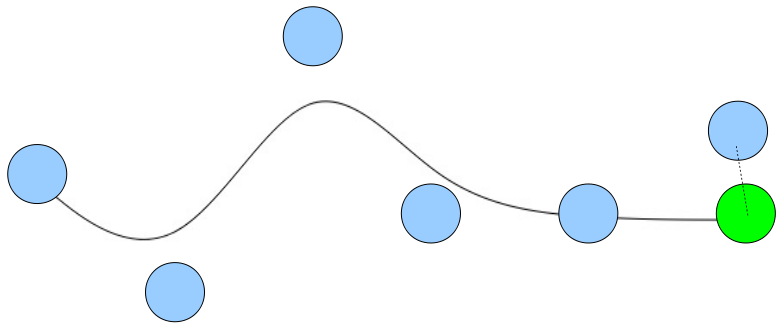
\includegraphics[width=0.6\textwidth]{julian-images/p2.png}
  \end{figure}
\begin{itemize}
 \item An identical scheme to Polynomial Extrapolation, but uses a spline curve for the polynomial.
 \item A Bezi\'er curve polynomial is used. These curves have better behaviour at high orders than Polynomial Extrapolation.
 \item This potentially leads to a better compression rate.
\end{itemize}
\end{frame}

\begin{frame}{Smallest Error Encoding}
\begin{figure}[h]
    \centering 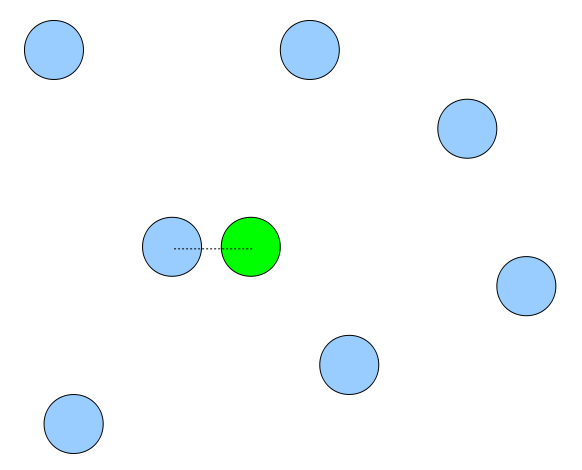
\includegraphics[trim = 0mm 0mm 0mm 25mm, clip, width=0.6\textwidth]{julian-images/p3.png}
  \end{figure}
\begin{itemize}
 \item Treats the memory as a databank of past atom positions.
 \item The atom is predicted to be at its closest previous position.
 \item The error is encoded as well as the time at which it was closest.
 \item Errors are kept as small as possible, but requires additional encoding overhead.
\end{itemize}
\end{frame}

\begin{frame}{Common Error and kNN Encoding}

\begin{itemize}
 \item Common Error Encoding
\begin{itemize}
 \item A scheme we invented to improve on the Smallest Error Encoding scheme.
 \item Heuristic functions are used for better compression.
 \item These heuristics use knowledge about which errors have been encoded most often.
 \item Still suffers from the additional encoding overhead as Smallest Error Encoding
\end{itemize}

\item k-Nearest Neighbour Encoding
\begin{itemize}
 \item Based on the machine learning algorithm called kNN.
 \item The scheme attempts to find patterns in the atom's positions.
 \item Errors are encoded from where it thinks that the atom should be.
 \item If a suitable pattern is found, it compresses well.
\end{itemize}
\end{itemize}
\end{frame}

\begin{frame}{Testing}
\begin{itemize}
 \item Several different molecular simulations were used. Specifically tested:
 \begin{itemize}
   \item Size of simulation: Number of atoms and frames.
   \item Coherency of motion: Temperature and simulation timestep.
   \item Simulation makeup: Water percentage.
 \end{itemize}
 \end{itemize}
\begin{figure}[h]
    \centering 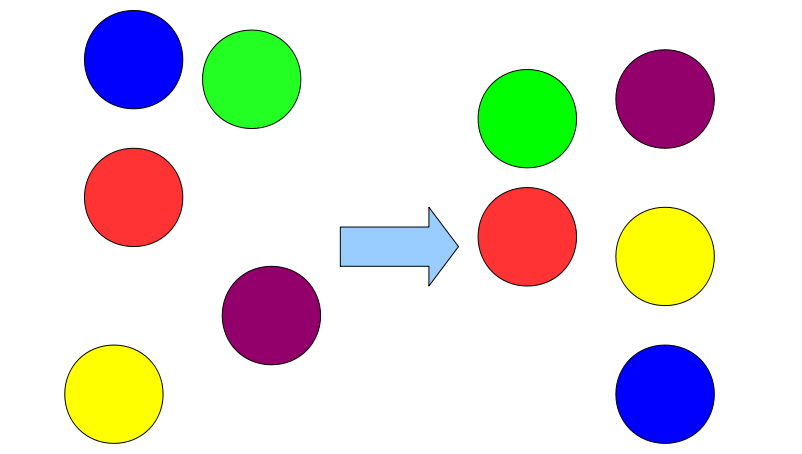
\includegraphics[width=0.5\textwidth]{julian-images/coherency.png}
  \caption{Simulations with low coherency of motion can have frames that appear unrelated to their previous frame.}
  \end{figure}
\end{frame}

\begin{frame}{Results}
\begin{figure}[h]
\centering 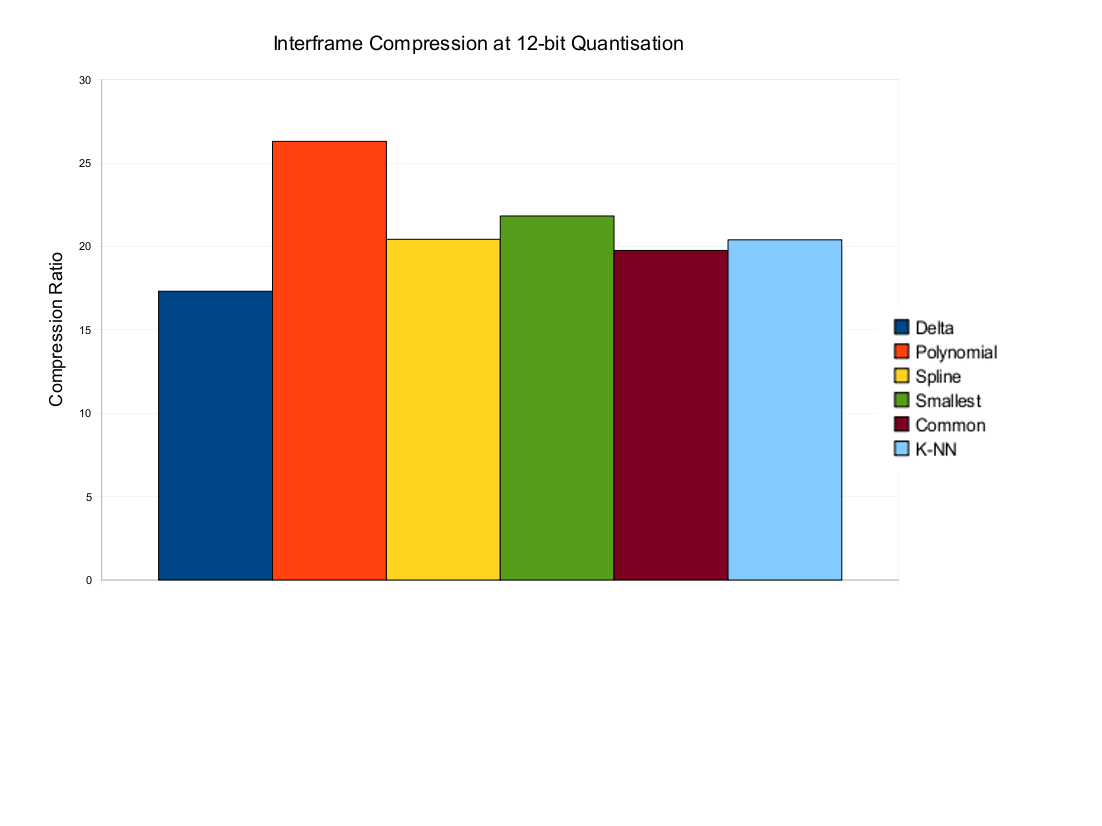
\includegraphics[trim = 10mm 60mm 10mm 5mm, clip,
  width=0.9\textwidth]{julian-images/interframe_results.png}
\end{figure}
\begin{itemize}
\item Our best scheme beats the current best scheme by approximately 20\%.
\end{itemize}
\end{frame}


\section{Conclusion}
\begin{frame}{Conclusion}{Research Answers}

  \begin{itemize}

  \item Visualisation and quantisation
    \begin{itemize}
    \item 8 bit quantisation is recommended for an acceptable level of
      quantisation.
    \item Applying filtering to reduce clutter effectively visualises large
      levels of detail.
    \end{itemize}

  \item Intraframe
    \begin{itemize}
    \item The more water in a simulation the better our scheme performs. This
      indicates that we are effectively exploiting the structure of water.
    \item Our scheme performs better than every other scheme tested.
    \item We compress and decompress in an efficient manner.
    \end{itemize}

  \item Interframe
    \begin{itemize}
      \item Interframe prediction can be used for compression.
      \item Our scheme performs better than existing compression scheme,
        especially in water-dominate simulations.
    \end{itemize}

  \end{itemize}
\end{frame}

\begin{frame}{Conclusion}

\begin{itemize}
 \item 8 bit quantisation recommended for visual fidelity.
 \item Exploiting the structure of water is a viable technique for compression.
 \item Exploiting the correlation between atom positions between frames is a viable technique for compression.
\end{itemize}

\end{frame}


\begin{frame}{Questions}
  \begin{center}
    \resizebox{0.1\textwidth}{!}{?}
  \end{center}
\end{frame}
% }}}

\end{document}

% LocalWords:  intraframe
